\documentclass{beamer}

\mode<presentation>
{
  \usetheme{default}      % or try Darmstadt, Madrid, Warsaw, ...
  \usecolortheme{default} % or try albatross, beaver, crane, ...
  \usefonttheme{default}  % or try serif, structurebold, ...
  \setbeamertemplate{navigation symbols}{}
  \setbeamertemplate{caption}[numbered]
} 

\usepackage[utf8]{inputenc}
% \usepackage[english,greek]{babel}
\usepackage{epstopdf}
% \newcommand{\en}{\selectlanguage{english}}
% \newcommand{\el}{\selectlanguage{greek}}
\usepackage{graphicx}
\graphicspath{ {./figures/} }
\usepackage{xcolor}
\usepackage{hyperref}

\usepackage{natbib}
\bibliographystyle{plainnat}

\title[]{PhD Status}
\author{Xanthos}
\institute{DSO \& IGN}
\date{\today}

\begin{document}

\begin{frame}
  \titlepage
\end{frame}

% Uncomment these lines for an automatically generated outline.
%\begin{frame}{Outline}
%  \tableofcontents
%\end{frame}

\section{Done}

\begin{frame}\frametitle{done to date ...}\framesubtitle{13/10/2021}

\begin{itemize}
    \item DORIS RINEX v3.x parser (tested)
    \item Sp3(c) parser (tested); works for all satellites
\end{itemize}

\end{frame}



\section{Immediate Goals}

\begin{frame}\frametitle{goals ...}\framesubtitle{13/10/2021}

\begin{itemize}
    \item Perform Sp3 (polynomial) interpolation (\textit{ready to some extend})
    \item Start implementing basic processing techniques from \cite{lemoine-2016}
\end{itemize}

\vspace{0.3cm}

\underline{Goal:} Estimate station coordinates using "fixed" orbits (from sp3)\\

Fine Points:
\begin{itemize}
    \item perform Doppler-like processing to remove ambiguity bias
    \item tropospheric delay (iers-2010 standards) -- \textit{maybe use a "static" model to begin with, e.g. Saastamoinen} --
    \item ionospheric delay (use iono-free LC)
    \item time, clocks and synchronization ...
    \item go for a Kalman filter (for estimation), not LS, so that we can later build on it
\end{itemize}

Could use more explicit references/documentation on DORIS processing

\end{frame}

\section{Implementation Details}

\begin{frame}\frametitle{RINEX observations}\framesubtitle{}
  DORIS RINEX files contain (as observables):
  \begin{itemize}
    \item L1 \& L2 phase data
    \item C1 \& C2 pseudo range data (only for time-tagging)
    \item W1 \& W2 power level data (data screening ?)
    \item Relative frequency data (?)
    \item P, T \& H meteorological data (later to be used for tropospheric dealy)
  \end{itemize}
  \vspace{.2cm}

  All observations include a complicated set of flags\\
  \vspace{.2cm}

  What about data screening/pre-processing? (e.g. Sigma-Clipping, see \citep{Ramanathan})
\end{frame}

\begin{frame}\frametitle{Parameters}\framesubtitle{SV coordinates}
    Extract satellite coordinates (or bettter yet state vector) from Sp3 files 
    using some kind of interpolation.\\
    \vspace{.2cm}
    
    At this point use polynomial interpolation using a (slightly modified) Neville's \citet{numrec3}
    method.\\
    \vspace{.2cm}
    
    Functions for reading/parsing Sp3 files are included in \href{https://github.com/xanthospap/sp3}{sp3}

    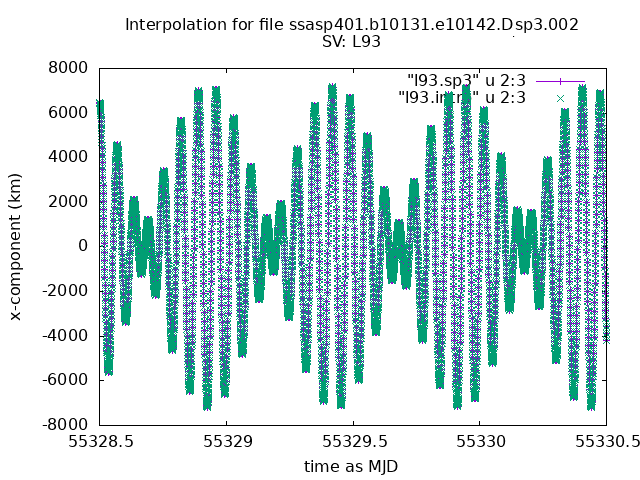
\includegraphics[scale=.4]{l93x}
\end{frame}

\begin{frame}\frametitle{Parameters}\framesubtitle{Station/Beacon coordinates}
    Extract station coordinates in ITRF2014\\
    \vspace{.3cm}

    Implementation ready (for all stations included in the corresponding .psd files).\\
    \vspace{.3cm}

\end{frame}

\begin{frame}\frametitle{Parameters}\framesubtitle{Time tagging}
    Quite complicated in DORIS ....
    \vspace{.3cm}

    Synchronize to TAI\\
    \vspace{.3cm}

  \begin{itemize}
      \item Use RINEX data (clock offsets) \textcolor{red}{use this first}
      \item Model clock using own model
  \end{itemize}
    \vspace{.3cm}

\end{frame}

\begin{frame}\frametitle{Parameters}\framesubtitle{Antenna PCO/PCV}
    Corrections for phase centre offset/variations\\
    \vspace{.3cm}

  Implemented for all ground antenna types,
  \begin{itemize}
      \item Alcatel
      \item StarecB/StarecC
  \end{itemize}
  \vspace{.3cm}

  Not yet implemented for SV's
  \vspace{.3cm}

\end{frame}

\bibliography{doris}

\end{document}
